\section{Exercise 1 3-Dimensional Boolean Functions}

\subsection{How many 3-dimensional Boolean functions are there}

Since a 3d boolean function are taking 3 boolean variables as argument. The number of unique combination of true/false values are $2^3 = 8$. Since there are two possible output for each of these true/false combinations, the total number of possible boolean functions can be calculated as $2^3 = 256$

\subsection{Count the number of symmetries of 3-dimensional Boolean functions that map 4 of the possible input patterns to 1.}

\begin{figure}
    \centering
    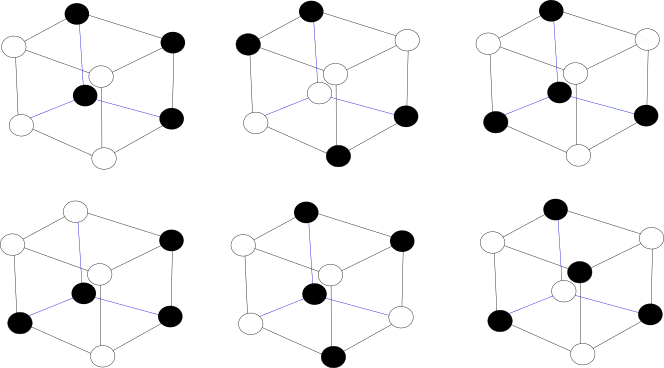
\includegraphics[scale=0.7]{FigSymmetry}
    \caption{Cubes describing the different symmetries}
    \label{fig:4tsym}
\end{figure}

the number of symmetries can be obtained by starting from one pattern of white coloured corners in the cube, and than iteratively switching positions between one white coloured, and black coloured corner in the cube.

The 6 Obtained symmetries can be found in figure \ref{fig:4tsym}.

\subsection{How many linearly separable 3-dimensional Boolean functions are there?}

One criterion for a boolean function to be linearly separable is that the corners in the cube that represents the true values needs have one edge connecting to at least another true value. It is also important for the cases where the function gives true on less than 5 unique inputs that none of the other true value is the others inverse. So if $(1,0,0)$ is mapped to true, than $(0,1,1)$ should not be true.

Using these criterions, we can calculate the numbers of linearly separable functions. case by case. However, note that if $f(v_1,v_2,v_3)$ is linearly separable, than $g(v_1,v_2,v_3) = \neg f(v_1,v_2,v_3)$ is also separable. Thus we need only to consider cases of 1,2,3 and 4 true outputs. 

Number of functions with only 1 input that gives true, is the number of corners, which is 8. For the case of 2, The only linearly separable function is the one where the true values covers a side of the cube, which there are 12 of on a cube. For the case of 3, the only symmetry of function is the one where three corners are connected by two sides. These can be situated by each corner, and "rotated" three times around the corners. Thus there are totally $3\cdot8 = 24$ number of these. There are two symmetries for the case of 4 that are linearly separable. Which is the first and third cube in figure \ref{fig:4tsym}. The first one is concentrated on a face of the cube, thus there are 6 of those. And the second symmetry are situated on a corner, thus there are 8. 5,6 and 7 are basically inverted functions of 1,2, and 3, thus these are the same amounts of these.

Summing these cases, as well as adding the functions that only gives true, or only false. We get $2 + 2(8 + 12 + 24) + 6 + 8 = 104$.